\section{Summary of Findings}

This section will give a brief summary of the baseline security issues found and solutions to said issues, based on the technical findings. For how these security issues were ranked and categorized, refer to "Appendix F - Risk Calculations"
\begin{longtable}{|l|p{10.5cm}|} 

\hline
\multicolumn{2}{|l|}{\textbf{OS Security issues discovered}}                              \\ \hline
\multirow{2}{*}{\textbf{File System Security}} & Some users where found to have more privileges than they really needed.      \\ \cline{2-2} 
                                               & A policy on what the users should have access to should be implemented. \\ & Risk: Medium \\ \hline



\multirow{2}{*}{\textbf{Password Policy}} &  After compromising the stored hashed passwords, we found that the passwords generated weak hashes and could easily be cracked.    \\ \cline{2-2} 
                                               & A policy to use longer passwords and passphrases is strongly adviced. It is also recommended to enforce the policy on every system. This will make it harder to bruteforce or crack the hashed passwords in case of compromise. \\ & Risk: Medium \\ \hline



\multirow{2}{*}{\textbf{Patching Policy}} & All the machines in the network was running outdated operating systems.    \\ \cline{2-2} 
                                               & Operating systems should always be updated to the latest version to avoid critical vulnerabilities. \\ & Risk: Medium \\ \hline



\multirow{2}{*}{\textbf{Trust Policy}} & Some users with high privileges where found to have undesirable behavior which the penetration team were able to exploit.    \\ \cline{2-2} 
                                               & Even users with extensive IT knowledge should not be blindly trusting. It is recommended to regularly conduct a trust review to make sure users can be trusted with their privileges. \\ & Risk: High. \\ \hline


\multirow{2}{*}{\textbf{Trust Policy}} & Some users with high privileges where found to have undesirable behavior which the penetration team were able to exploit.    \\ \cline{2-2} 
                                               & Even users with extensive IT knowledge should not be blindly trusting. It is recommended to regularly conduct a trust review to make sure users can be trusted with their privileges. \\ & Risk: High. \\ \hline


\multirow{2}{*}{\textbf{Trust Policy}} & Some users with high privileges where found to have undesirable behavior which the penetration team were able to exploit.    \\ \cline{2-2} 
                                               & Even users with extensive IT knowledge should not be blindly trusting. It is recommended to regularly conduct a trust review to make sure users can be trusted with their privileges. \\ & Risk: High. \\ \hline

\end{longtable}


\begin{longtable}{|l|p{10.5cm}|} 
\hline
\multicolumn{2}{|l|}{Web Server Security}                              \\ \hline

\multirow{2}{*}{\textbf{Patching Policy}} & The version of the web server running was found to be vulnerable to multiple exploits. These include shellshock (CVE-2014-6271), SQLi exploitation and Path Traversal exploitation. These vulnerabilities can cause high impact.    \\ \cline{2-2} 
                                               & The web server is highly accessible from the outside, which significantly increases the threat. All vulnerabilities should be patched as soon as a patch is available. It is also highly recommended that a IDPS is implemented to detect and prevent attackers from accessing the systems. \\ & Risk: High \\ \hline

\end{longtable}

\newpage
Group 3 found that there are multiple highly critical issues as summarized in the table below.
\begin{table}[h]
\centering
\begin{tabular}{|l|l|l|}
\hline
Low & Medium & High \\ \hline
0   & 3      & 4    \\ \hline
\end{tabular}
\caption{Risk Table}
\end{table}

\begin{figure}[h!]
  \centering
    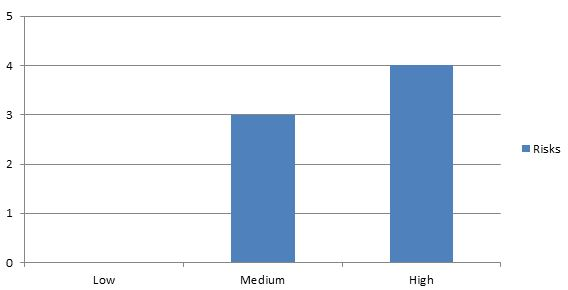
\includegraphics{./Graphics/riskchart.JPG}
 \caption{Risk compare chart.}
\end{figure}
